\subsection{Képfeldolgozás, konvolúció, élkeresés, szegmentálás, alakfelismerés.}

\textbf{Open CV Computer Vision Library}
\begin{itemize}
    \item open source computer vision library: gépi látást segítő nyílt forráskódú könyvtár
    \item több, mint 2500 optimalizált algoritmus
    \item képek adatainak feldolgozása
    \item objektumok felismerése
    \item gépi tanulás támogatása
\end{itemize}

\textbf{Képi adatok feldolgozása:}
\begin{itemize}
    \item színfényesség hisztogram
    \begin{center}
        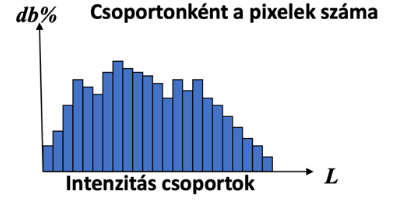
\includegraphics[width=0.6\textwidth]{res/imgs/info_24_color_histogram.png}
    \end{center}
    \item képminőségek
    \begin{center}
        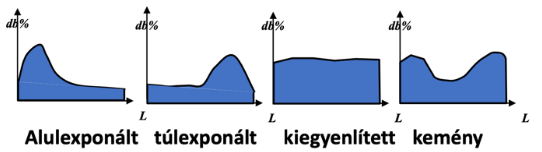
\includegraphics[width=0.95\textwidth]{res/imgs/info_24_image_qualities.png}
    \end{center}
\end{itemize}

\textbf{Képhibák javítása:}
\begin{itemize}
    \item Konvolúció
    \begin{itemize}
        \item egy képpont intenzitása a képpont és a környezete intenzitásának súlyozott összege
        \begin{equation*}
            q(k,l) = t \otimes g(k,l) = \sum_{r=-R}^{R} \sum_{s=-S}^{S} t(r,s) \cdot g(k+r, l+s)
        \end{equation*}
        \item $g$ - a képpont eredeti világossága
        \item $q$ - a képpont új világossága
        \item $t$ - a súlyok (az operator), rendszerint páratlan számú sort és oszlopot tartalmaz
    \end{itemize}
    \item Szűrések (lágyítás):
    \begin{itemize}
        \item elmosás
        \begin{itemize}
            \item a képpont és a környezete világosságának átlaga -- lágyít
            \begin{equation*}
                Mag = \frac{1}{\text{ksize.width} \cdot \text{ksize.height}} \cdot \begin{bmatrix}
                    1 & 1 & \dots & 1 \\
                    1 & 1 & \dots & 1 \\
                    \dots & \dots & \dots & \dots \\
                    1 & 1 & \dots & 1
                \end{bmatrix}
            \end{equation*}
        \end{itemize}
        \item Gauss elmosás
        \begin{itemize}
            \item Gauss-eloszlás (haranggörbe) alapján számoljuk
            \item A normális eloszlás haranggörbéje \quad $G(x) = \frac{1}{\sigma \sqrt{2\pi}} e^{-\frac{x^2}{2\sigma^2}}$
            \item Két dimenzióban a magfüggvény \quad $G(x,y) = K e^{-\frac{x^2}{2\sigma^2} - \frac{y^2}{2\sigma^2}}$
            \item $\sigma$ a szórás, 0 a várható érték
        \end{itemize}
        \item medián (rank) szűrés (nem lineáris)
        \begin{itemize}
            \item egypontos hibákra, az adott pont a környezetének mediánja lesz
        \end{itemize}
    \end{itemize}
\end{itemize}

\textbf{Képek élesítése:}
\begin{itemize}
    \item életlenség eltávolítása
    \begin{itemize}
        \item éles kép = 1,5 * kép - 0,5 * blur(kép)
    \end{itemize}
    \item bilaterális szűrés
    \begin{itemize}
        \item zajokat eltávolítja, éleket megtartja
        \item élesítés, ahol nagy a szórás
        \item \verb|bilateralFilter()|
    \end{itemize}
\end{itemize}

\textbf{Élkeresés:}
\begin{itemize}
    \item vízszintes és függőleges irányú változásokat első és magasabbrendű differencia képzésével emelhetjük ki
    \item változás sebességének vizsgálata (gradiens)
    \begin{center}
        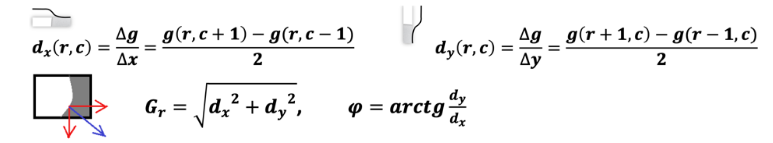
\includegraphics[width=0.95\textwidth]{res/imgs/info_24_gradients.png}
    \end{center}
    \item élkeresés a változás gyorsulása alapján (Laplace)
    \begin{equation*}
        \begin{split}
            \partial_x^2 g(k,l) &= \partial_x g(k,l) - \partial_x g(k,l-1) = g(k,l+1) - g(k,l) - [g(k,l) - g(k,l-1)] = \\
            &= g(k,l+1) - 2 \cdot g(k,l) + g(k,l-1) \\
            \partial_y^2 g(k,l) &= \partial_y g(k,l) - \partial_y g(k-1,l) = g(k+1,l) - g(k,l) - [g(k,l) - g(k-1,l)] = \\
            &= g(k+1,l) - 2 \cdot g(k,l) + g(k-1,l)
        \end{split}
    \end{equation*}
    \item élkeresés Canny módszerével
    \begin{itemize}
        \item Gauss zajszűrés
        \item szürkeárnyalatos kép
        \item vízszintes és függőleges gradiens komponensek (irány kerekítve 45 fokra)
        \item nem maximum eltüntetés (kiemelkedő marad)
        \item gradiens küszöb
    \end{itemize}
    \begin{center}
        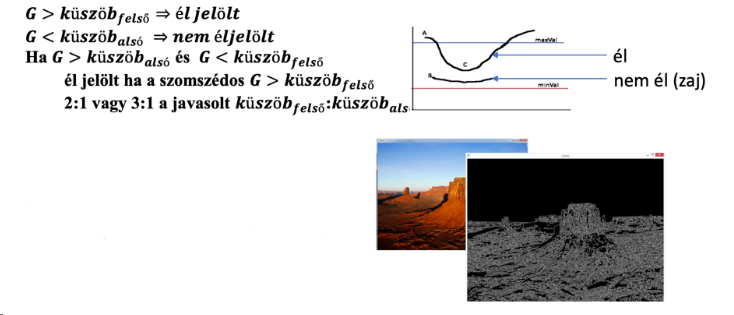
\includegraphics[width=0.9\textwidth]{res/imgs/info_24_canny_edge.png}
    \end{center}
\end{itemize}

\textbf{Szegmentálás:}
\begin{itemize}
    \item szegmentálás, csoportosítás, rendezés érzékelés alapján
    \item összetartozó jellemzők összegyűjtése, csoportosítása
    \item szegmentálás felülről lefelé (Top-down): közös ismert objektum hasonló pixeleinek keresése
    \item szegmentálás lentről felfelé (Bottom-up): azonos jellegű pixelek gyűjtése pixelből indítva
\end{itemize}
\begin{center}
    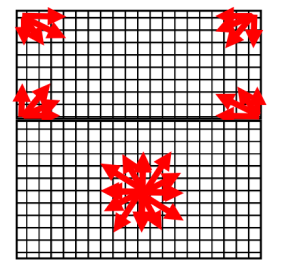
\includegraphics[width=0.4\textwidth]{res/imgs/info_24_segmentation_grid.png}
\end{center}

\textbf{Globális szegmentálás:}
\begin{itemize}
    \item globális szegmentálás küszöbértékekkel
    \begin{itemize}
        \item Top-down
        \item ha a hasonló intenzitású keresett elem és a háttér között nagy a kontraszt
    \end{itemize}
    \item \verb|threshold()|
    \begin{center}
        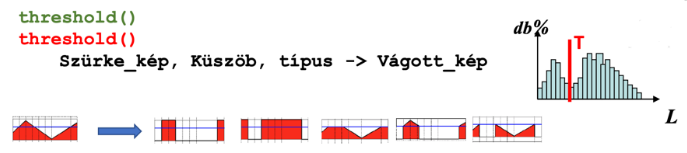
\includegraphics[width=0.95\textwidth]{res/imgs/info_24_global_threshold.png}
    \end{center}
    \item Otsu módszere
    \begin{itemize}
        \item Top-down
    \end{itemize}
    \begin{center}
        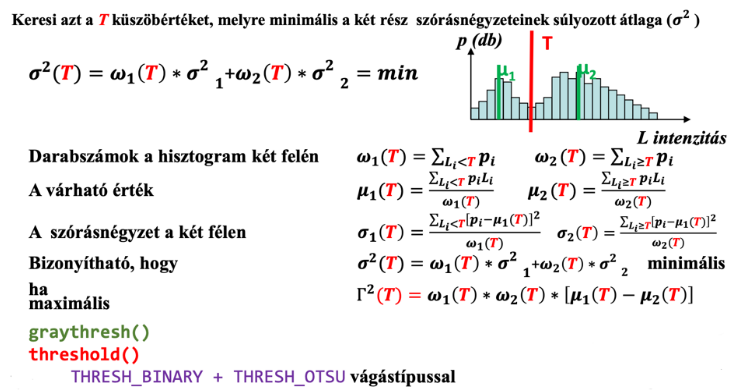
\includegraphics[width=0.95\textwidth]{res/imgs/info_24_otsu_method.png}
    \end{center}
    \item \verb|graythresh()|, \verb|threshold()| (THRESH\_BINARY + THRESH\_OTSU)
    \item Isodata algoritmus – Iterativ Self-Organizing Data Analysis Technique
    \begin{itemize}
        \item Top-down
    \end{itemize}
    \begin{center}
        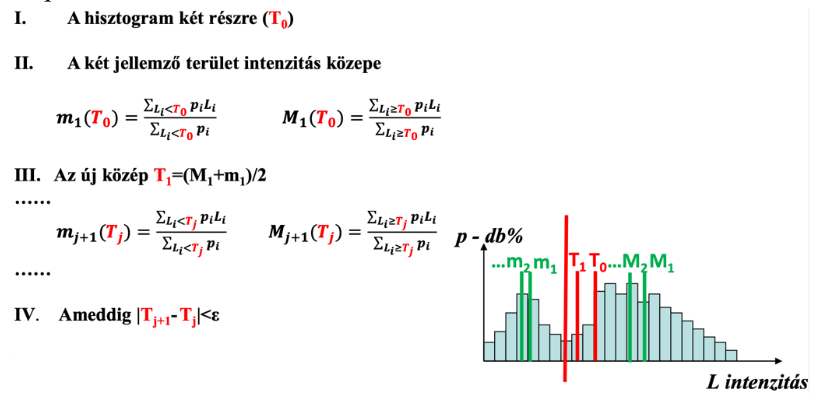
\includegraphics[width=0.95\textwidth]{res/imgs/info_24_isodata_algorithm.png}
    \end{center}
\end{itemize}

\textbf{Lokális szegmentálás – Bottom up:}
\begin{itemize}
    \item adaptív szegmentálás küszöbértékekkel
    \begin{itemize}
        \item átlaggal vág
    \end{itemize}
    \item elárasztás statisztikával
    \begin{itemize}
        \item $P$ a vizsgált pont intenzitása, körülötte $T$ tartományban $N$ szomszédos pont
        \item $T$ tartományban $p_i$ a pontok intenzitása
        \item $\mu = \frac{1}{N} \sum_T p_i$ (az intenzitás várható értéke)
        \item $\sigma^2 = \frac{1}{N-1} \sum_T (p_i - \mu)^2$ (az intenzitás korrigált tapasztalati szórásnégyzete)
        \item $\tau = \sqrt{\frac{N}{N+1}} * \frac{(P - \mu)^2}{\sigma^2}$
        \item $\tau \le K$ küszöbszám akkor szomszédos P pont a régióhoz tartozik.
    \end{itemize}
    \item elárasztás vágóélekkel
\end{itemize}

\textbf{Alakfelismerés:}
\begin{itemize}
    \item alakfelismerés sablonillesztéssel
    \begin{equation*}
        r = \frac{ \sum_{i=1}^n (sz_{1_i} - \overline{sz}_1) \cdot (sz_{2_i} - \overline{sz}_2) }{ \sqrt{ \sum_{i=1}^n (sz_{1_i} - \overline{sz}_1)^2 \cdot \sum_{i=1}^n (sz_{2_i} - \overline{sz}_2)^2 } }
    \end{equation*}
    \begin{itemize}
        \item A korrelációs együttható - a várható értéktől való eltérések szorzata (covariancia) osztva a szórások szorzatával - két tetszőleges elemhalmaz közötti lineáris kapcsolat nagyságát és irányát jellemzi
        \item A minta ($sz_1$) korrelációja a kép részleteivel ($sz_2$)
        \item A legjobb illeszkedést az a képrészlet adja, amelyre a korrelációs együttható a legnagyobb.
        \item \verb|vision.TemplateMatcher()|
        \item \verb|matchTemplate()| (Kép, minta -> korrelációs térkép)
    \end{itemize}
    \begin{center}
        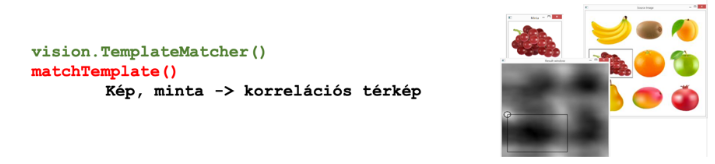
\includegraphics[width=0.8\textwidth]{res/imgs/info_24_template_matching.png}
    \end{center}
    \item alakfelismerés Hough transzformációval
    \begin{itemize}
        \item egyenesek:
        \begin{center}
            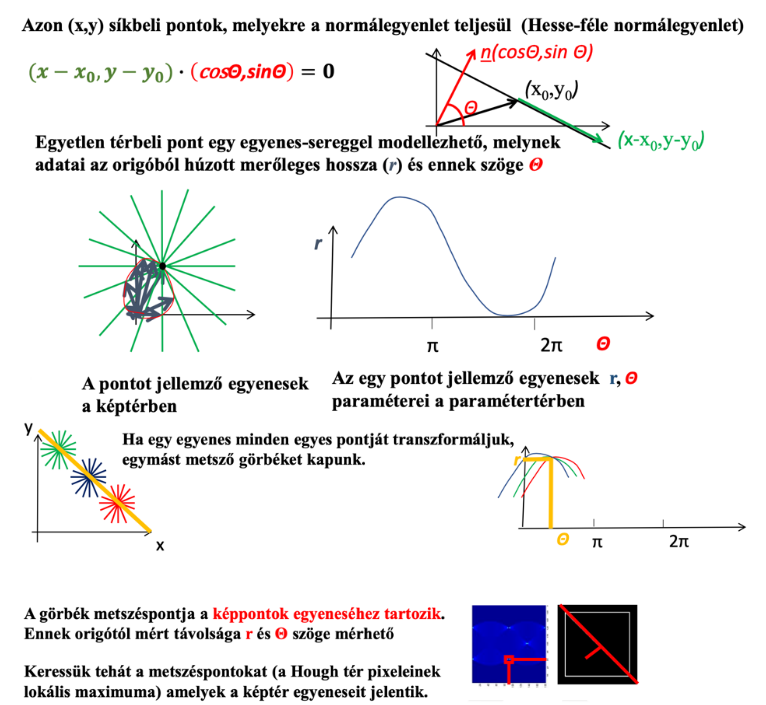
\includegraphics[width=0.95\textwidth]{res/imgs/info_24_hough_lines.png}
        \end{center}
        \begin{itemize}
            \item lényege, hogy a polárkoordinátával több egyenes leírható, mely átmegy egy adott ponton
            \item ha felrajzoljuk grafikonon ezeket az egyenleteket r-re $\Theta$ függvényében, akkor az adott egyenesen lévő pontokat transzformáljuk, akkor a görbék egymást metszeni fogják, méghozzá azokban a polárkoordinátákban, melyek leírják a képtér egyeneseit
        \end{itemize}
        \item körök:
        \begin{center}
            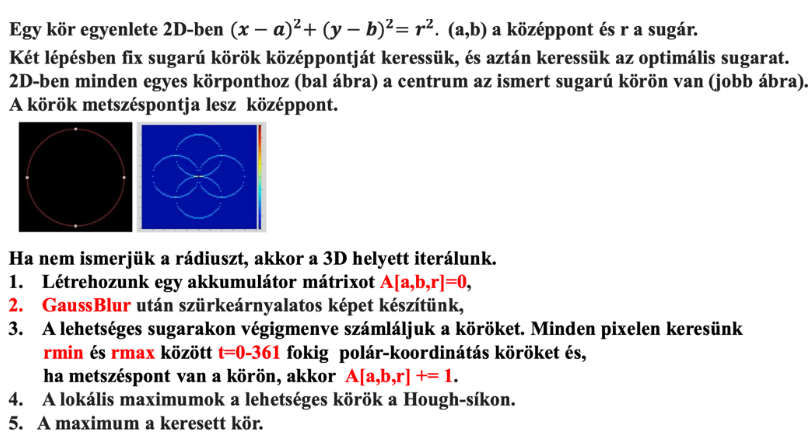
\includegraphics[width=0.95\textwidth]{res/imgs/info_24_hough_circles.png}
        \end{center}
    \end{itemize}
\end{itemize}